\documentclass[UTF8,a4paper,12pt]{article}

\usepackage[version=3]{mhchem} % Package for chemical equation typesetting
\usepackage{ctex}
\usepackage{siunitx} % Provides the \SI{}{} and \si{} command for typesetting SI units
\usepackage{graphicx} % Required for the inclusion of images
\usepackage{natbib} % Required to change bibliography style to APA
\usepackage{amsmath} % Required for some math elements
\usepackage{enumitem}
\usepackage{indentfirst}

\usepackage[top=2cm, bottom=2cm, left=2cm, right=2cm]{geometry}
\usepackage{algorithm}
\usepackage{algorithmicx}
\usepackage{algpseudocode}

\renewcommand{\labelenumi}{\alph{enumi}.} % Make numbering in the enumerate environment by letter rather than number (e.g. section 6)
\floatname{algorithm}{算法}
\renewcommand{\algorithmicrequire}{\textbf{输入:}}
\renewcommand{\algorithmicensure}{\textbf{输出:}}

\usepackage{listings}

\usepackage{tikz}
\usetikzlibrary{shapes.geometric, arrows}

% \usepackage{times} % Uncomment to use the Times New Roman font
%----------------------------------------------------------------------------------------
%	DOCUMENT INFORMATION
%----------------------------------------------------------------------------------------

\begin{document}

\begin{titlepage}
    \begin{center}
        \phantom{Start!}
    	  \vspace{2cm}
        \center{\zihao{1} 中山大学数据科学与计算机学院}
        \center{\zihao{1} 计算机科学与技术专业-人工智能}
        \center{\zihao{1} 本科生实验报告}
        \center{(2018-2019学年秋季学期)}
        {
            \setlength{\baselineskip}{40pt}
            \vspace{1cm}
            \zihao{-2}
            \center{
                \begin{tabular}{cc}
              	学\qquad 号:& \underline{~~~~~~16337113~~~~~~}  \\
              	姓\qquad 名:& \underline{~~~~~~~劳马东~~~~~~~}  \\
                教学班级:   & \underline{~~~~~教务2班~~~~~}  \\
              	专\qquad 业:& \underline{~~~~~~~~~超算~~~~~~~~}  \\
              	\end{tabular}
            }
        }
    \end{center}
\end{titlepage}

\section{实验题目}
\par 实现ID3,C4.5,CART三种决策树。不要求实现连续型数据的处理,不要求实现剪枝。
\section{实验内容}
\subsection{算法原理}
\subsubsection{决策树}
\par 决策树是一棵多叉树,它通过执行一系列测试达到决策。树中内部节点代表对输入属性$A_i$的值的
一个测试(如年龄),从结点射出的分支代表属性$A_i$的可能值(如$\ge 18$岁),叶节点代表一种决策。
\par 分类决策树模型是一种描述对实例进行分类的决策树,叶节点表示一个类。用决策树分类,从根节点开始,
对实例的某一特征进行测试,根据测试结果,将实例分配到其子节点;这时,每一个子节点对应着该特征的一个取值。
如此递归地对实例进行测试并分配,直到达到叶节点。最后将实例分到叶节点的类中。
\subsubsection{决策树的建树过程}
\begin{enumerate}[itemindent=0.5em,label=\arabic*、]
  \item 初始化\\创建根结点,它拥有全部数据集和特征。
  \item 选择特征\\遍历当前结点的数据集和特征,根某种原则选择一个特征。
  \item 划分数据\\根据这个特征的取值,将当前数集划分为若干子集。
  \item 创建结点\\为每个子数据集创建一个子结点,并删去选中的特征。
  \item 递归建树\\对每个子结点,回到第2步,直到达到边界条件,则回溯。\\
  递归边界条件:
  \begin{itemize}
    \item 剩余样例属于同一类C,该节点标记为C类叶节点,返回C;
    \item 无样例,此时返回一个缺省值,该值是构造其父节点用到的所有样例中得票最多的类$C_p$
    ,该节点标记为$C_p$类叶节点;
    \item 无属性可选择,根据多数投票原则选出剩余样例的类别$C_v$,该节点标记为$C_v$类叶节点,
    返回$C_v$。
  \end{itemize}
  \item 完成建树\\叶子结点采用多数投票的方式判定自身类别。
\end{enumerate}
\subsubsection{特征选择指标}
\par 假设数据集(X, Y)的子数据集个数为n,每个子数据集为$(X_i, Y_i)(i \in [0, n))$,属性集F的每个属性为$F_j$,
则属性$F_j$在指标M上所得的分数为:
\begin{equation}
  \mathop{S(Y|F_j)}_{F_j \in F} = \sum_{i=0}^{n-1}(\frac{|Y_i|}{Y} \times M(Y_i))
\end{equation}

\begin{enumerate}[itemindent=0.5em,label=\arabic*、]
  \item 错误率\\
  对于$Y_i$根据多数投票原则得到其类别$C_i$,错误率计算$Y_i$中出现错误的频率。公式如下:
  \begin{equation}
    M(Y_i)= \frac{|\{y_k \in Y_i: y_k \neq C_i\}|}{|Y_i|}
  \end{equation}
  我们希望最优属性使得错误率最小,即:
  \begin{equation}
    \begin{aligned}
      best(F) &= \mathop{\arg\min}_{F_j \in F}{S(Y|F_j)}\\
      &= \mathop{\arg\max}_{F_j \in F}{[S(Y) - S(Y|F_j)]}
    \end{aligned}
  \end{equation}
  \item 信息增益\\
  信息增益采用熵计算,熵是随机变量不确定性的度量,其计算公式为:
  \begin{equation}
    M(Y_i) = H(Y_i) = -\sum_{k}p(y_k)\log _2p(y_k)
  \end{equation}
    $p(v_k)$表示$v_k$在V上的频率。
  随机变量A的信息增益表示A对Y的不确定性的减小程度,公式为:
  \begin{equation}
    I(A) = H(Y) - H(Y|A)
  \end{equation}
我们希望最优属性使得Y的不确定性最小,即:
\begin{equation}
  \begin{aligned}
    best(F) &= \mathop{\arg\max}_{F_j \in F}{[H(Y) - H(Y|F_j)]} \\
    &= \mathop{\arg\max}_{F_j \in F}{[S(Y) - S(Y|F_j)]}\\
  \end{aligned}
\end{equation}
  \item 信息增益率\\
  信息增益的方法偏向于找出分支多的属性作为最优属性,因为分支越多代表不确定性越小,信息增益就越大。
  然而选择分支多的属性容易造成过拟合,因此该方法对其进行改进,在信息增益的基础之上乘上一个惩罚参数。
  特征取值较多时,惩罚参数较小;特征取值较少时,惩罚参数较大。该参数为特征的熵的倒数。公式如下:
  \begin{equation}
    \begin{aligned}
      best(F) &= \mathop{\arg\max}_{F_j \in F}{\frac{H(Y) - H(Y|F_j)}{H(F_j)}}\\
      &= \mathop{\arg\max}_{F_j \in F}{\frac{S(Y) - S(Y|F_j)}{S(F_j)}}
    \end{aligned}
  \end{equation}

  \item 基尼系数\\
  基尼系数原本是用以衡量一个国家或地区居民收入差距的指标,介于0-1之间。基尼系数越大,表示不平等程度越高。
  对于一个随机变量,基尼系数代表其取值的差异程度,计算公式如下:
  \begin{equation}
      M(Y_i) = G(Y_i) = \sum_{k}p(y_k) \times (1 - p(y_k)) = 1 - \sum_{k}p(y_k)^2
  \end{equation}
  我们希望选择的最优属性使Y取值的差异程度最小,即:
  \begin{equation}
    \begin{aligned}
      best(F) &= \mathop{\arg\min}_{F_j \in F}{G(Y|F_j)}\\
      &= \mathop{\arg\min}_{F_j \in F}{S(Y|F_j)}\\
       &= \mathop{\arg\max}_{F_j \in F}{[S(Y) - S(Y|F_j)]}\\
    \end{aligned}
  \end{equation}
\end{enumerate}
\par 从以上分析可以看出,特征选择的公式可以统一化为一个公式:
\begin{equation}
    best(F) = \mathop{\arg\max}_{F_j \in F}{\frac{S(Y) - S(Y|F_j)}{punishment}}
\end{equation}
\par 对于信息增益率方法,$punishment=H(F_j)$,其余方法为1。
\newpage
\subsection{伪代码}
\begin{enumerate}[itemindent=0.5em,label=\arabic*、]
  \item 决策树建树过程基本框架
  \begin{algorithm}
        \begin{algorithmic}[1] %每行显示行号
            \Require 训练集X,训练集y,父节点$parent$,分支的取值$brach$
            \Function {$build\_tree$}{$X, y, parent, brach$}
                \State $F \gets feature(X)$
                \State $root \gets Node(brach, parent)$
                \If {$X \ is \  empty$}
                  \State $root.label \gets parent.label$
                \ElsIf {$F \ is \ empty$}
                  \State $root.label \gets vote(X)$
                \ElsIf {$is\_same(y)$}
                  \State $root.label \gets y[0]$
                \Else
                \State $root.label \gets vote(y)$
                \State $S_y \gets M(y)$
                \For {each ${F_j} \in F$}
                  \State $S_j \gets 0$
                  \For {each $(F_{ji},X_i,y_i) \in divide(F_j,X,y)$}
                    \State $S_j \gets S_j + \frac{|y_i|}{|y|} \times M(y_i)$
                  \EndFor
                  \State $S_j \gets \frac{S_y - S_j}{punishment}$
                  \State $S_{best}, F_{best} \gets \max(S_{best}, F_{best}, S_j, F_j)$
                \EndFor
                \State $root.feature \gets F_{best}$
                \State // 根据所选属性划分数据集
                \For {each $(branch,X_i,y_i) \in divide(F_{best},X,y)$}
                  \State $sub\_tree = build\_tree(X_i, y_i, root, branch)$ // 递归建树
                  \State $root.add\_child(sub\_tree)$
                \EndFor
                \EndIf
                \State \Return{$root$}
            \EndFunction
        \end{algorithmic}
    \end{algorithm}
\end{enumerate}

\newpage
\subsection{关键代码}
\begin{enumerate}[itemindent=0.5em,label=\arabic*、]
  \item 特征选择:遍历所有属性(编号为数字),根据该属性划分数据集为若干子数据集,计算
  子数据集在某种指标上的得分,最后求这些子数据集得分的均值。如果该指标带有惩罚参数,得分
  均值需要乘上惩罚参数。
  \begin{figure}[h]
  \begin{center}
  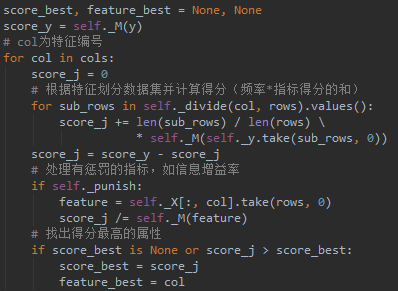
\includegraphics[width=0.8\textwidth]{p4.png} % Include the image placeholder.png
  \caption{特征选择}
  \end{center}
  \end{figure}
  \item 数据集划分与递归:选择出最优属性后,需要将其从属性集合中删除,并创建一个内部结点,
  代表一种划分方法。该节点的类标签由数据集根据多数投票原则得出,当在测试集上无相应分支
  时返回这个内部结点的类标签。根据最优属性划分数据集递归建树,值得注意的地方是cols需要传
  副本而不是本身,否则在回溯时cols的值将发生改变。
  \begin{figure}[h]
  \begin{center}
  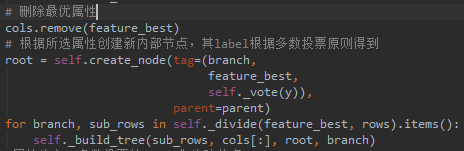
\includegraphics[width=0.8\textwidth]{p5.png} % Include the image placeholder.png
  \caption{数据集划分与递归}
  \end{center}
  \end{figure}
  \item 预测:预测的过程就是顺着决策树不断匹配的过程。取测试数据在对应属性上的值,如果有匹配的分支
  则进入分支继续重复该过程,否则返回结点的类标签。
  \begin{figure}[h]
  \begin{center}
  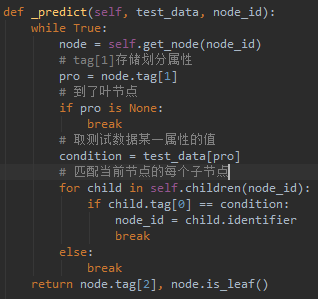
\includegraphics[width=0.8\textwidth]{p6.png} % Include the image placeholder.png
  \caption{预测}
  \end{center}
  \end{figure}
\end{enumerate}

\section{优化\&创新}
\begin{enumerate}[itemindent=0.5em,label=\arabic*、]
  \item 数据集划分优化
  \par \qquad 数据集的划分涉及到许多次拷贝,例如,要将$m \times n$的X分成$[0, a)$、$[a, b)$、$[b, m)$
  的三部分,若采用简单的划分方式,即返回$X[0:a]$、$X[a:b]$、$X[b:n]$,将会出现非常多的拷贝,
  时间复杂度为$(O(m \times n))$, 尤其是当n较大时,拷贝将会成为瓶颈。同理,选择了最优属性之后将其对应的列从
  矩阵中删除也会引起很多拷贝。
  \par \qquad 其实,只需要记录当前子树对应的行的集合,以此表示子数据集;记录对应的列的集合,以此表示可用属性。
  在划分时对行的集合进行划分而不是对数据集本身划分,就能将时间复杂度降低为$O(m\log m + n\log n)$。

  \begin{figure}[h]
  \begin{center}
  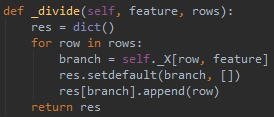
\includegraphics[width=0.6\textwidth]{p7.png}
  \caption{按属性划分优化}
  \end{center}
  \end{figure}

\end{enumerate}
\section{实验结果及分析}
\subsection{实验结果展示示例}
\begin{enumerate}[itemindent=0.5em,label=\arabic*、]
  \item 数据集样本\\
  挑选实验数据前20行作为训练集,21-25行作为测试集。
  \begin{figure}[h]
  \begin{center}
  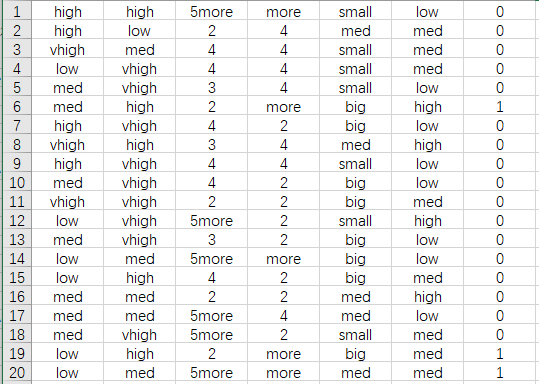
\includegraphics[width=0.6\textwidth]{p8.png}
  \caption{训练集}
  \end{center}
  \end{figure}

  \begin{figure}[h]
  \begin{center}
  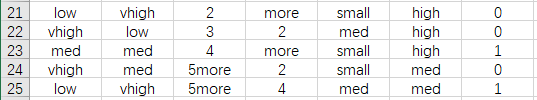
\includegraphics[width=0.6\textwidth]{p9.png}
  \caption{测试集}
  \end{center}
  \end{figure}
  \item 建树过程\\
  以CART树为例,第一次递归根节点有全部数据集,各个属性计算得到的基尼系数为$0:0.219, 1:0.2, 2:0.203, 3:0.12, 4:0.23, 5:0.225$,
  其中最小的是属性3,因此选择属性3作为划分标准。属性3有三种取值:取值为2的有第6, 9, 10, 11, 12, 14, 15, 17行,y值全部为0;
  取值为4的有第1, 2, 3, 4, 7, 8, 16行,y值全部为0;取值为more的有第0, 5, 13, 18, 19行,计算得到属性0、1、2、4、5的基尼系数
  分别为0.267, 0.467, 0.267, 0.267, 0,最小的是属性5。继续以属性5划分数据集,以此类推,过程正确。
  \begin{center}
    \begin{tabular}{c|c|c|c|c|c}
    \hline
    层数 & 分支 & 数据集/行 & 基尼系数 & 选择 & 类\\
    \hline
    1	& - & [0, 1, 2, ... , 17, 18, 19] & 0.219, 0.2, 0.203, 0.12, 0.230, 0.225 & 3 & -\\
    2	& 4 & [1, 2, 3, 4, 7, 8, 16] & - & - & 0\\
    2	& 2 & [6, 9, 10, 11, 12, 14, 15, 17] & - & - & 0\\
    2	& more & [0, 5, 13, 18, 19] & 0:0.267, 1:0.467, 2:0.267, 4:0.267, 5:0 & 5 & -\\
    3	& low & [0, 13] & - & - & 0\\
    3	& high & [5] & - & - & 1\\
    3	& med & [18, 19] & - & - & 1\\
    \hline
    \end{tabular}
  \end{center}

  \item 决策树建树结果
  \thispagestyle{empty}
  % 定义基本形状
  \tikzstyle{results}=[ellipse ,text centered,draw=black]
  \tikzstyle{decisions} =[rectangle, rounded corners,text centered, draw = black]
  % 箭头形式
  \tikzstyle{arrow} = [-,>=stealth]

  \begin{center}
    \begin{tikzpicture}[node distance=2cm]
    %定义具体形状和相关位置
    \node[decisions](rootnode){属性3};
    \node[results,below of=rootnode,xshift=-2.5cm](result1){0};
    \node[decisions,below of=rootnode](touchpoint){属性5};
    \node[results,below of=rootnode,xshift=2.5cm](result2){0};

    \node[results,below of=touchpoint,xshift=-2cm](result3){1};
    \node[results,below of=touchpoint](result4){0};
    \node[results,below of=touchpoint,xshift=2cm](result5){1};
    %连接形状
    \draw [arrow] (rootnode) -- node [left,font=\small] {2} (result1);
    \draw [arrow] (rootnode) -- node [left,font=\small] {more} (touchpoint);
    \draw [arrow] (rootnode) -- node [right,font=\small] {4} (result2);
    \draw [arrow] (touchpoint) -- node [left,font=\small] {high} (result3);
    \draw [arrow] (touchpoint) -- node [left,font=\small] {low} (result4);
    \draw [arrow] (touchpoint) -- node [right,font=\small] {med} (result5);
    \end{tikzpicture}
  \end{center}

  \item 决策结果\\
  对于测试集第0行,其属性3的值为more,进入more子树;其属性5的值为high,预测为1,符合;\\
  对于测试集第1行,其属性3的值为2,预测为0,符合;\\
  以此类推,预测结果符合预期;
  \begin{center}
    \begin{tabular}{cc}
    \hline
    测试数据/行 & 预测标签\\
    \hline
    21 & 1\\
    22 & 0\\
    23 & 1\\
    24 & 0\\
    25 & 0\\
    \hline
    \end{tabular}
  \end{center}
\end{enumerate}

\subsection{评测指标展示及分析}
\begin{enumerate}[itemindent=0.5em,label=\arabic*、]
  \item 准确率
  \item 优化前后训练时间对比
\end{enumerate}
\section{思考题}
\begin{itemize}
  \item 决策树有哪些避免过拟合的方法?
  \item C4.5相比于ID3的优点是什么,C4.5又可能有什么缺点?
  \item 如何用决策树来进行特征选择(判断的重要性)?
\end{itemize}
\end{document}
